%%
%% This is file `sample-sigchi.tex',
%% generated with the docstrip utility.
%%
%% The original source files were:
%%
%% samples.dtx  (with options: `sigchi')
%% 
%% IMPORTANT NOTICE:
%% 
%% For the copyright see the source file.
%% 
%% Any modified versions of this file must be renamed
%% with new filenames distinct from sample-sigchi.tex.
%% 
%% For distribution of the original source see the terms
%% for copying and modification in the file samples.dtx.
%% 
%% This generated file may be distributed as long as the
%% original source files, as listed above, are part of the
%% same distribution. (The sources need not necessarily be
%% in the same archive or directory.)
%%
%% The first command in your LaTeX source must be the \documentclass command.
\documentclass[sigchi]{acmart}

\usepackage{xcolor}
\usepackage{amssymb}
\usepackage{amsmath}
\usepackage{amsthm}
\usepackage{graphicx}

%%
%% \BibTeX command to typeset BibTeX logo in the docs
\AtBeginDocument{%
  \providecommand\BibTeX{{%
    \normalfont B\kern-0.5em{\scshape i\kern-0.25em b}\kern-0.8em\TeX}}}

%% Rights management information.  This information is sent to you
%% when you complete the rights form.  These commands have SAMPLE
%% values in them; it is your responsibility as an author to replace
%% the commands and values with those provided to you when you
%% complete the rights form.
%\setcopyright{acmcopyright}
%\copyrightyear{2018}
%\acmYear{2018}
%\acmDOI{10.1145/1122445.1122456}

%% These commands are for a PROCEEDINGS abstract or paper.
%\acmConference[Woodstock '18]{Woodstock '18: ACM Symposium on Neural
%  Gaze Detection}{June 03--05, 2018}{Woodstock, NY}
%\acmBooktitle{Woodstock '18: ACM Symposium on Neural Gaze Detection,
%  June 03--05, 2018, Woodstock, NY}
%\acmPrice{15.00}
%\acmISBN{978-1-4503-9999-9/18/06}


%%
%% Submission ID.
%% Use this when submitting an article to a sponsored event. You'll
%% receive a unique submission ID from the organizers
%% of the event, and this ID should be used as the parameter to this command.
%%\acmSubmissionID{123-A56-BU3}

%%
%% The majority of ACM publications use numbered citations and
%% references.  The command \citestyle{authoryear} switches to the
%% "author year" style.
%%
%% If you are preparing content for an event
%% sponsored by ACM SIGGRAPH, you must use the "author year" style of
%% citations and references.
%% Uncommenting
%% the next command will enable that style.
%%\citestyle{acmauthoryear}

%%
%% end of the preamble, start of the body of the document source.
\begin{document}

%%
%% The "title" command has an optional parameter,
%% allowing the author to define a "short title" to be used in page headers.
\title{Interactive Visualization of Neural Network Activities}

%%
%% The "author" command and its associated commands are used to define
%% the authors and their affiliations.
%% Of note is the shared affiliation of the first two authors, and the
%% "authornote" and "authornotemark" commands
%% used to denote shared contribution to the research.
\author{Zijian Li}
%\email{trovato@corporation.com}
%\orcid{1234-5678-9012}
%\author{G.K.M. Tobin}
%\authornotemark[1]
%\email{webmaster@marysville-ohio.com}
\affiliation{%
  \institution{University of Washington}
}

\author{Callin Switzer}
\affiliation{%
  \institution{University of Washington}
}

\author{Yue Zhao}
\affiliation{%
  \institution{University of Washington}
}

\author{Zhengde Zhao}
\affiliation{%
  \institution{University of Washington}
}
%%
%% By default, the full list of authors will be used in the page
%% headers. Often, this list is too long, and will overlap
%% other information printed in the page headers. This command allows
%% the author to define a more concise list
%% of authors' names for this purpose.
%\renewcommand{\shortauthors}{Trovato and Tobin, et al.}

%%
%% The abstract is a short summary of the work to be presented in the
%% article.
\begin{abstract}
  A clear and well-documented \LaTeX\ document is presented as an
  article formatted for publication by ACM in a conference proceedings
  or journal publication. Based on the ``acmart'' document class, this
  article presents and explains many of the common variations, as well
  as many of the formatting elements an author may use in the
  preparation of the documentation of their work.
\end{abstract}

%%
%% The code below is generated by the tool at http://dl.acm.org/ccs.cfm.
%% Please copy and paste the code instead of the example below.
%%

%%
%% Keywords. The author(s) should pick words that accurately describe
%% the work being presented. Separate the keywords with commas.
\keywords{Neural networks, Data Visualization, Interactive}

%%
%% This command processes the author and affiliation and title
%% information and builds the first part of the formatted document.
\maketitle

\section{Introduction}

\subsection{Background}

%% The primary parameter given to the ``\verb|acmart|'' document class is the {\itshape template style} which corresponds to the kind of publication or SIG publishing the work. This parameter is enclosed in square brackets and is a part of the {\verb|documentclass|} command:
%%\begin{verbatim}
%%  \documentclass[STYLE]{acmart}
%%\end{verbatim}

%%Journals use one of three template styles. All but three ACM journals use the {\verb|acmsmall|} template style:
%%\begin{itemize}
%%\item {\verb|acmsmall|}: The default journal template style.
%%\item {\verb|acmlarge|}: Used by JOCCH and TAP.
%%\item {\verb|acmtog|}: Used by TOG.
%%\end{itemize}

%%The majority of conference proceedings documentation will use the {\verb|acmconf|} template style.
%%\begin{itemize}
%%\item {\verb|acmconf|}: The default proceedings template style.
%%\item{\verb|sigchi|}: Used for SIGCHI conference articles.
%%\item{\verb|sigchi-a|}: Used for SIGCHI ``Extended Abstract'' articles.
%%\item{\verb|sigplan|}: Used for SIGPLAN conference articles.
%%\end{itemize}

Insects like moths have very simple brains, yet they are capable of precise and subtle flying maneuvers, which involve complex fluid dynamics. They generate locomotor force by activating the flight muscles to move their wings, and the aerodynamic forces and torques it generates enable they to preform various flying behaviors including fast forward, odor plume tracking, hovering in front of flowers, decelerating upon approach and conpensating for enrionmental perturbations \cite{Stevenson1665}  \cite{Willis1991}
. To understand how moths control their flight is already by itself interesting, not to mention that  bio-inspired flapping wings system has potential application to micro air vehicles according to Chen in \cite{Chen_2018}. 

\emph{\color{blue} [Picture of a realistic Moth]}

Multiple recent researchers has targeted this question. In \cite{Hedrick3114}, the authors treated this question as an inverse problem, where the input of the system is the initial position, initial velocity, targeting position and targeting velocity while the output of the system is the wing motion. They developed an aerodynamic model illustrating how a particular motion in the wings of a moth could result in a kinetic motion. In \cite{Dyhr1523}, they found that not only the wings but also the shape of the body plays an important role in a moth's flight control. New variables such as the angle of the body of the moth were introduced into the model. Further study has also shown that structural deformation also affects flapping wing energetics, see \citep{Jankauski_2018}. Nevertheless, to solve the inverse problem of flight control is intrinsically difficult. It involves solving a highly nonlinear dynamically system. 

On the other side, people has developed theory to solve dynamical systems with machine learning techniques. For example see \cite{WilliamsRD15}. Moreover, recent study show some very successful examples in solving model based motion control problem with deep learning neural networks. For instance, see \cite{Kalakrishnan} and \cite{Tassa} for legged robot locomation and \cite{Mellinger} for aggressive control of autonomous quadrotors. With these successes, people are also looking into such a deep learning solution to the dynamical system of moth flight control.

\subsection{Neural Network \& Visualization}

Dr. Switzer, a researcher in the Biology Department of University of Washington, and his colleagues developed several deep learning neural networks in order to solve the moth flight control problem. More specifically, they want to know the following. Suppose I am a moth and I know where I am and where I want to go, how do I get there? To answer this, they first built up a virtual moth. With this virtual moth, they simulated a dataset consisting of the actions the moth is taking and its resulting kinetic motion. After that, they trained several different neural networks, with different scales, using this dataset and lastly they evaluated the predictions by the neural network. It turns out that the best of their model is able to recreate a large share of the variance of the dependent variables in this model, with $r^2 > 0.999$.

\emph{\color{blue} [Picture as PPT page 10]}

\emph{\color{blue} [Picture prediction result]}


Now with these neural networks, we are able to generate an action for a particular intended motion that a moth is to take. The next step is to see how meaningful information we are able to extract from this neural network solution.



\section{Methods}
Neural networks are a special type of graph networks, which are highly organized in their structures. For a feedforward neural network used in this study, nodes in the graph are divided into layers, and the group of nodes in each layer only connect with nodes in the adjacent layers. \cite{bischof1992visualization} described the visualization of feedforward neural networks, which aligns the position of the nodes according to their layer number. The following Figure \ref{ffnn} shows the structure of one example of a fully-connected feedforward neural network used in the virtual moth modeling. The figure also shows a typical way of visualizing such a neural network: nodes are aligned onto different lines, using the horizontal position to encode their layers. Weights are then drawn as lines connected each two nodes in adjacent layers.  

\begin{figure}[h]
  \centering
  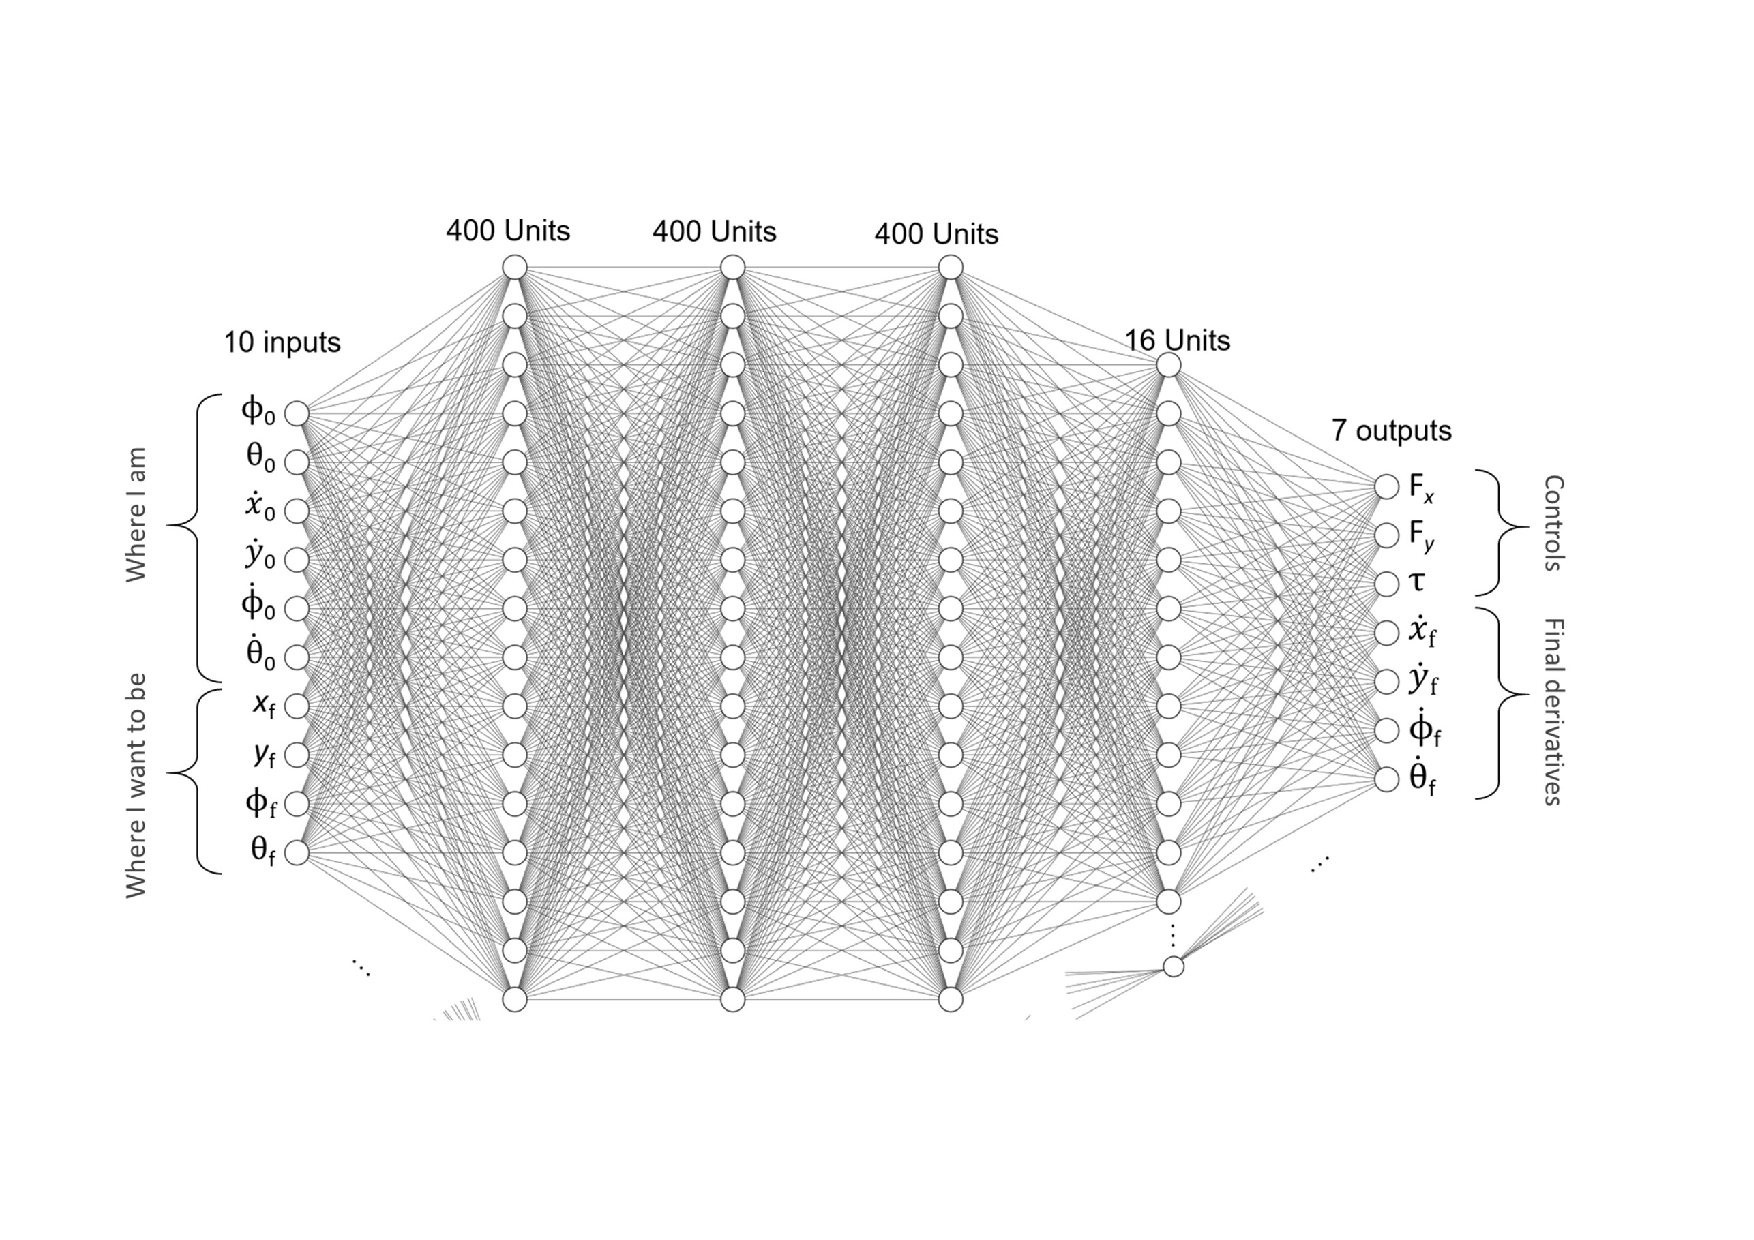
\includegraphics[width=\linewidth]{ffnn.pdf}
  \caption{Feedforward Neural Network}
  \Description{A example of a feedforward neural network structure used in the modeling of a virtual moth. The network is fully-connected between adjacent layers.} 
  \label{ffnn}
\end{figure}

The above visualization of a neural network is clear in understanding the model structure, but has some drawbacks as well. First of all, this visualization is static, which does not respond to the changes in the network, such as activation on the nodes, cutting of of weight connections. Secondly, it is bad under scaling, and can only serve as a conceptual illustration. For example, there are 400 units in the middle layers, but the visualization is incapable of showing all of them, thus it is impossible to show the complete activities and weights architecture in the network. The alignment of all the nodes in one layer, while adjustable to different network structures is a big problem. Lastly, such visualization is only suitable to simple constructions of neural networks such as the feedforward network. With the rapid development of new network structures nowadays, such as the recurrent neural network based on \cite{rumelhart1988learning}, a simple static framework for visualizing all types of neural networks is impossible. We tackles these problems with the following methods.

\subsection{Computational Graph Construction}
For a fully-connected feedforward neural network, the connections between each two adjacent layers are in the form of a bipartite graph, which can be represented by a weight matrix $W$, where $W_{ij}$ represents the weight between the $i$-th node in the previous layer and the $j$-th nodes in the next layer. The weight matrices are also the typical data structure of storing a neural network. To consider an arbitrary construction of neural network, however, we consider the most general super-class of neural networks, the computational graph model. The directed graph 
\[
G = (V, E)
\]
consists of a set of nodes $V$ and the set of edges $E$. Each edge $e \in E$ goes from a node $v_1 \in V$ to another node $v_2 \in V$. In the neural network, the elements in the graph have their properties as follows:
\begin{align*}
& v \in V: \ \mbox{node ID}\ i, \ \mbox{layer number}\ l, \ \mbox{activation value}\ u, \\
& e \in E: \ \mbox{source}\ i, \ \mbox{target}\ j, \ \mbox{weight}\ w.
\end{align*}
Note that the activation value $u$ on each nodes is determined not only by the neural network itself, but also depends on the inputs to the network. Therefore, the network construction should be real-time in response to interactive input selection. To solve this problem, we construct the graph together with all  the element properties listed above. For the feedforward neural network case in our study, we implement the forward pass algorithm that starts from the input layers, and iterates throughout the whole network to the output layer. 

Since many neural networks are highly pruned in our study, a large portion of weights are zeros or close to zero. It is undesirable to show these edges, and thus we throw away these edges in the construction phase. This would help largely reduce the amount of computation in the following visualization stage. In addition to edge trimming, we also walk through the network after construction, and throw away any node which is not connected to any edge. This way the trimmed network is kept as a connected graph, in preparation for the force-directed layout in the next stage.

\subsection{Force Directed Layout}
In stead of aligning the nodes according to the layers into strict lines, we use the force directed layout scheme \citep{fruchterman1991graph}. Each node $v_i$ is regarded as a charged particle with charge $q_i$. Each two nodes $v_i$ and $v_j$ repel each other with the force
\[
F = \frac{q_i q_j}{d_{ij}^2}.
\]
Each edge $e$ is considered as a spring, applying the attracting force to the nodes it connects:
\[
F = k(L - d_{ij}).
\]
Besides, each node in motion is subject to air resistance
\[
F = -b v_i.
\]
At each time step, the forces acting on each node are calculated, which are then integrated to update its velocity and position. In our system, we implement the force directed layout scheme in d3-force, which uses a velocity Verlet numerical integrator for simulating physical forces on particles. 

To show the layered structure of the neural network better, we apply external force field to form a beeswarm plot. Similar to plotting nodes in different layers onto different X-positions, we apply attractive X-forces to nodes in each layer towards the corresponding X-position. A constant attractive force in the Y direction is also applied to ensure reasonable vertical scale of the plot. The whole graph is also attracted to the center of the plot. To make the algorithm scalable to different sizes of networks, we choose the charges and forced according to the total number of nodes in the graph:
\[
F_X \sim \frac{1}{|V|^2}, \quad q \sim \frac{1}{|V|}.
\]




%\section{Rights Information}
%
%Authors of any work published by ACM will need to complete a rights
%form. Depending on the kind of work, and the rights management choice
%made by the author, this may be copyright transfer, permission,
%license, or an OA (open access) agreement.
%
%Regardless of the rights management choice, the author will receive a
%copy of the completed rights form once it has been submitted. This
%form contains \LaTeX\ commands that must be copied into the source
%document. When the document source is compiled, these commands and
%their parameters add formatted text to several areas of the final
%document:
%\begin{itemize}
%\item the ``ACM Reference Format'' text on the first page.
%\item the ``rights management'' text on the first page.
%\item the conference information in the page header(s).
%\end{itemize}
%
%Rights information is unique to the work; if you are preparing several
%works for an event, make sure to use the correct set of commands with
%each of the works.


\section{Tables}

The ``\verb|acmart|'' document class includes the ``\verb|booktabs|''
package --- \url{https://ctan.org/pkg/booktabs} --- for preparing
high-quality tables.

Table captions are placed {\itshape above} the table.

Because tables cannot be split across pages, the best placement for
them is typically the top of the page nearest their initial cite.  To
ensure this proper ``floating'' placement of tables, use the
environment \textbf{table} to enclose the table's contents and the
table caption.  The contents of the table itself must go in the
\textbf{tabular} environment, to be aligned properly in rows and
columns, with the desired horizontal and vertical rules.  Again,
detailed instructions on \textbf{tabular} material are found in the
\textit{\LaTeX\ User's Guide}.

Immediately following this sentence is the point at which
Table~\ref{tab:freq} is included in the input file; compare the
placement of the table here with the table in the printed output of
this document.

\begin{table}
  \caption{Frequency of Special Characters}
  \label{tab:freq}
  \begin{tabular}{ccl}
    \toprule
    Non-English or Math&Frequency&Comments\\
    \midrule
    \O & 1 in 1,000& For Swedish names\\
    $\pi$ & 1 in 5& Common in math\\
    \$ & 4 in 5 & Used in business\\
    $\Psi^2_1$ & 1 in 40,000& Unexplained usage\\
  \bottomrule
\end{tabular}
\end{table}

To set a wider table, which takes up the whole width of the page's
live area, use the environment \textbf{table*} to enclose the table's
contents and the table caption.  As with a single-column table, this
wide table will ``float'' to a location deemed more
desirable. Immediately following this sentence is the point at which
Table is included in the input file; again, it is
instructive to compare the placement of the table here with the table
in the printed output of this document.

\begin{table*}
  \caption{Some Typical Commands}
  \label{tab:commands}
  \begin{tabular}{ccl}
    \toprule
    Command &A Number & Comments\\
    \midrule
    \texttt{{\char'134}author} & 100& Author \\
    \texttt{{\char'134}table}& 300 & For tables\\
    \texttt{{\char'134}table*}& 400& For wider tables\\
    \bottomrule
  \end{tabular}
\end{table*}


\section{Figures}

The ``\verb|figure|'' environment should be used for figures. One or
more images can be placed within a figure. If your figure contains
third-party material, you must clearly identify it as such, as shown
in the example below.
\begin{figure}[h]
  \centering
 % \includegraphics[width=\linewidth]{sample-franklin}
  \caption{1907 Franklin Model D roadster. Photograph by Harris \&
    Ewing, Inc. [Public domain], via Wikimedia
    Commons. (\url{https://goo.gl/VLCRBB}).}
  \Description{The 1907 Franklin Model D roadster.}
\end{figure}

Your figures should contain a caption which describes the figure to
the reader. Figure captions go below the figure. Your figures should
{\bfseries also} include a description suitable for screen readers, to
assist the visually-challenged to better understand your work.

Figure captions are placed {\itshape below} the figure.

\subsection{The ``Teaser Figure''}

A ``teaser figure'' is an image, or set of images in one figure, that
are placed after all author and affiliation information, and before
the body of the article, spanning the page. If you wish to have such a
figure in your article, place the command immediately before the
\verb|\maketitle| command:
\begin{verbatim}
  \begin{teaserfigure}
    \includegraphics[width=\textwidth]{sampleteaser}
    \caption{figure caption}
    \Description{figure description}
  \end{teaserfigure}
\end{verbatim}




\section{SIGCHI Extended Abstracts}

The ``\verb|sigchi-a|'' template style (available only in \LaTeX\ and
not in Word) produces a landscape-orientation formatted article, with
a wide left margin. Three environments are available for use with the
``\verb|sigchi-a|'' template style, and produce formatted output in
the margin:
\begin{itemize}
\item {\verb|sidebar|}:  Place formatted text in the margin.
\item {\verb|marginfigure|}: Place a figure in the margin.
\item {\verb|margintable|}: Place a table in the margin.
\end{itemize}

%%
%% The acknowledgments section is defined using the "acks" environment
%% (and NOT an unnumbered section). This ensures the proper
%% identification of the section in the article metadata, and the
%% consistent spelling of the heading.
\begin{acks}
To Robert, for the bagels and explaining CMYK and color spaces.
\end{acks}

%%
%% The next two lines define the bibliography style to be used, and
%% the bibliography file.
\bibliographystyle{ACM-Reference-Format}
\bibliography{bib}

%%
%% If your work has an appendix, this is the place to put it.
\appendix

\section{Research Methods}


\subsection{Part Two}

Etiam commodo feugiat nisl pulvinar pellentesque. Etiam auctor sodales
ligula, non varius nibh pulvinar semper. Suspendisse nec lectus non
ipsum convallis congue hendrerit vitae sapien. Donec at laoreet
eros. Vivamus non purus placerat, scelerisque diam eu, cursus
ante. Etiam aliquam tortor auctor efficitur mattis.

\section{Online Resources}

Nam id fermentum dui. Suspendisse sagittis tortor a nulla mollis, in
pulvinar ex pretium. Sed interdum orci quis metus euismod, et sagittis
enim maximus. Vestibulum gravida massa ut felis suscipit
congue. Quisque mattis elit a risus ultrices commodo venenatis eget
dui. Etiam sagittis eleifend elementum.

Nam interdum magna at lectus dignissim, ac dignissim lorem
rhoncus. Maecenas eu arcu ac neque placerat aliquam. Nunc pulvinar
massa et mattis lacinia.

\end{document}
\endinput
